\documentclass[journal]{IEEEtran}
\usepackage{amsmath,amsfonts}
\usepackage{algorithm,algpseudocode}
\usepackage{array}
\usepackage[caption=false,font=normalsize,labelfont=sf,textfont=sf]{subfig}
\usepackage{textcomp}
\usepackage{stfloats}
\usepackage{url}
\usepackage{verbatim}
\usepackage{graphicx}
\usepackage[bookmarksnumbered, colorlinks, plainpages]{hyperref}
\usepackage[dvipsnames]{xcolor}
%\hyphenation{op-tical net-works semi-conduc-tor IEEE-Xplore}

\usepackage{balance}
\begin{document}
\title{Final Report of the Group Project for CS5351\\
\colorbox{yellow}{\textit{!We Need Project Title: An informative title!}}
}

\input{private/author}


%\markboth{Journal of \LaTeX\ Class Files,~Vol.~18, No.~9, September~2020}%
%{How to Use the IEEEtran \LaTeX \ Templates}

\markboth{Final Report of the Group Project for CS5351, November~2023}%
{Title of the Project TBD.}

\maketitle

\begin{abstract}
This document describes blablabal....
abstract to be consideration.

\textit{Requirements: needs (150 words) }

\end{abstract}

\begin{IEEEkeywords}
Software Engineering, Software Testing, Computer Science, Software Maintainance, Software Debug.
\end{IEEEkeywords}


\section{Introduction}
\IEEEPARstart{T}{his} collaborative effort reflects the team's dedication to creating tools that aid software engineers in improving code quality by detecting code smells. 

The following sections provide an in-depth look at the project's background, the proposed solution, the software development process, evaluation results, and concluding remarks.

\textbf{(about 1-1.5 pages)}

\section{Related Work}
\noindent The 2nd Part is Related Work, something that related with our work. like A\cite{feng2023efficiency,10.1109/ICSE48619.2023.00167,10.1145/3510003.3510105}, B\cite{9793896}, C\cite{9793896}, D\cite{10.1145/2025113.2025179}, E\cite{yandrapally2023carving} and others\cite{9402052,10172611,10190433} .....

\textit{Requirements: Present your fact finding about existing solutions toward solving the problem stated in the section on Introduction}. 

\textbf{(about 1 page)}

\section{Preliminaries}
\noindent The 3rd part is Preliminaries.
blablabal....

The Preliminaries section lays the foundation for the reader by presenting essential technical background information. It encompasses a summary of the knowledge required to understand the developed tools, focusing on code smells, their significance, and existing tools in the domain. This section aims to equip the reader with the necessary context to comprehend the subsequent discussion.

\textit{Requirements: Summary of the technical background information necessary to follow your idea and solution.} 

\textbf{(about 1-2 pages)}

\section{Solution}
\noindent The 4th part is Solution.
blablabal....

The Solution section articulates the team's approach to addressing code smells using an innovative tool. This part of the report encompasses detailed descriptions, algorithms, figures, and code listings that elucidate the inner workings of the solution. The team provides an example walkthrough to illustrate how the tool functions, emphasizing its relevance to topics covered in the CS5351 course.

\textit{Requirements: Present your solution, probably with algorithms, figures, code listing, and an example walkthrough to assist you in presenting your solution. Relate the content to each topic covered in CS5351.}

\textbf{(2-3 pages)}


\subsection{Multi-Platform}

To maximize accessibility, our tool is designed for deployment in diverse scenarios, with a focus on both user-friendly web access and a simplified GUI for desktop users. This approach aligns with the principles of usability and adaptability emphasized in software engineering.

\subsubsection{B/S-Based Application}

Our primary deployment targets a Browser/Server (B/S) architecture, providing users with a seamless and user-friendly experience. This platform-independent approach ensures that developers can easily access and utilize our tool without the need for specific operating systems or installations. This aligns with software engineering emphasis on web-based technologies and their relevance in modern software development.

\subsubsection{Desktop GUI}

Recognizing the diversity in developer preferences and environments, we also provide a straightforward Graphical User Interface (GUI) for desktop users. This option ensures that our tool caters to developers who may prefer a local installation or work within specific desktop environments. This versatility resonates with the adaptability concepts covered in software engineering.

\subsection{DevOps Integration}

In keeping with contemporary software engineering practices, our tool is deployed using robust DevOps practices, aligning with the DevOps principles covered in software engineering.

\subsubsection{Cloud Deployment on Microsoft Azure}

We leverage Microsoft Azure for cloud deployment, offering scalability, reliability, and a range of services that enhance the overall performance of our tool. This choice aligns with software engineering's coverage of cloud computing and its role in modern software development.

\subsubsection{Containerization with Docker}

To enhance portability and consistency across different environments, we utilize Docker for containerization. This allows our tool and its dependencies to be packaged together, ensuring that it runs consistently on various platforms. This aligns with software engineering's coverage of containerization and its impact on software deployment.

\begin{algorithm}[hbt!]
    \caption{Scalability Model}\label{alg:Scalabilitymodel}
    \begin{algorithmic}
    
    \Require $Deployment\ Definition$
  
    \State Initialization($Deployment\ Definition$) 

    \Repeat
        \State Monitoring($sys\_Status$)
        \State $New\ Definition$ $\gets$ Replica\_Calculation($sys\_Status$)
        \State Initialization($New\ Definition$) 
    \Until{$Done$}
    
    \end{algorithmic}
  \end{algorithm}

\subsubsection{Kubernetes for Scalability}

Ensuring our tool's robustness and scalability, we employ Kubernetes for container orchestration in algorithm \ref{alg:Scalabilitymodel}. This choice aligns with software engineering's exploration of scalable architectures and their significance in handling diverse workloads efficiently.

\begin{figure}[!t]
\centering

\includegraphics[width=2.5in]{figures/k8slogo.png}
\caption{Employing DevOps Techniques.}
\label{fig:k8slogo}
\end{figure}


\section{Software Process}
\noindent The 5th part is Software Process..

The Software Process section documents the team's activities throughout the project, highlighting the achievements of each sprint. Each sprint is elaborated on in two pages, capturing the essence of the tasks undertaken, challenges faced, and milestones achieved. Additionally, the section includes a burndown chart, offering a visual representation of project progress throughout its duration.


\textit{Requirements: Document the activities and the achieved of each sprint in 2 pages (a total of 2*N pages for a project with N sprints). Include the burndown chart for the whole project.}



\textbf{(each sprint in 2 pages (a total of 2*N pages for a project with N sprints))}

\section{Evaluation}
\noindent The 6th part is Evaluation...


The Evaluation section summarizes the verification and evaluation processes applied to the solution. It outlines how the team gauged the effectiveness of the tool in solving the identified code smell problems. Special attention is given to scalability considerations, comparing the results to existing tools in the software engineering landscape.


\textit{Requirements: Summarize what you have verified or evaluated your solution to have solved the problem stated in the report, and compare to the results of existing tools}

\textbf{(2-5 pages)}


\subsection{Security}
The evaluation dives into the scalability of the developed tools, exploring their performance in handling varying codebase sizes. This section utilizes equations and figures to demonstrate scalability metrics. A comparative analysis with existing tools further validates the tool's efficacy.


\subsection{Scalability}

Scalability is a critical aspect of our code smell detection tool, as it determines its ability to handle diverse and large-scale software projects efficiently. The evaluation involves several key components:

\subsubsection{Test Scenarios}

We conducted scalability tests across a spectrum of software projects, ranging from small-scale applications to large enterprise-level systems. This diversity ensures that our tool's performance is assessed under realistic conditions.

\subsubsection{Metrics}

To quantify scalability, we measured the tool's performance based on key metrics, including execution time, memory usage, and response time. These metrics provide insights into how well the tool handles increasing codebase sizes without significant degradation in performance.

\subsubsection{Comparison with Existing Tools}

To contextualize our results, we compared the scalability of our tool with existing code smell detection tools in the industry. This comparative analysis offers a benchmark for understanding the tool's performance relative to established solutions.

\subsubsection{Scalability Equations}

We utilized scalability equations to model the tool's performance as the size of the codebase increases. These equations help predict how the tool will scale in different scenarios and provide valuable insights for future users.

\subsubsection{Parallel Processing}

Incorporating principles covered in software engineering, our tool utilizes parallel processing techniques to enhance scalability. This involves efficiently distributing the workload across multiple processing units, mitigating bottlenecks and improving overall performance.

\subsubsection{Dynamic Scaling}

Our tool employs dynamic scaling mechanisms, adjusting resource allocation based on the size and complexity of the codebase being analyzed. This adaptive approach ensures optimal performance across a wide range of scenarios.

\subsubsection{Results and Analysis}

The scalability evaluation yielded promising results, showcasing our tool's ability to efficiently handle diverse codebases. Execution times remained within acceptable limits even as project sizes increased. Memory usage demonstrated stability, and response times were consistently low.

Comparison with existing tools highlighted the competitive scalability of our solution, positioning it as a viable option for developers working on projects of varying scales.

\subsubsection{Future Considerations}

To ensure continued scalability as software projects evolve, we outline plans for future enhancements. This includes ongoing optimization efforts, monitoring for potential bottlenecks, and incorporating feedback from users to address specific scalability challenges in real-world scenarios.



\section{Conclusion}
\noindent The 7th part is Conclusion...

The Conclusion section provides a concise recap of the main achievements, encompassing the software development process, activities, techniques, deliverables, the tool itself, and noteworthy best practices. Additionally, the team outlines areas for future work, indicating the potential evolution of the tools and any further enhancements planned.

\textit{Requirements: Recap the main achievement (process, activities, techniques, deliverables, tool, people, and best practice) and future work.}

\textbf{(about 1 page)}


\newpage
\section*{Word Count Testing}
\noindent The Part is for testing how many word perpage...

Repeat Repeat Repeat Repeat Repeat Repeat Repeat Repeat Repeat Repeat Repeat Repeat Repeat Repeat Repeat Repeat Repeat Repeat Repeat Repeat Repeat Repeat Repeat Repeat Repeat Repeat Repeat Repeat Repeat Repeat Repeat Repeat Repeat Repeat Repeat Repeat Repeat Repeat Repeat Repeat Repeat Repeat Repeat Repeat Repeat Repeat Repeat Repeat Repeat Repeat Repeat Repeat Repeat Repeat Repeat Repeat Repeat Repeat Repeat Repeat Repeat Repeat Repeat Repeat Repeat Repeat Repeat Repeat Repeat Repeat Repeat Repeat Repeat Repeat Repeat Repeat Repeat Repeat Repeat Repeat Repeat Repeat Repeat Repeat Repeat Repeat Repeat Repeat Repeat Repeat Repeat Repeat Repeat Repeat Repeat Repeat Repeat Repeat Repeat Repeat Repeat Repeat Repeat Repeat Repeat Repeat Repeat Repeat Repeat Repeat Repeat Repeat Repeat Repeat Repeat Repeat Repeat Repeat Repeat Repeat Repeat Repeat Repeat Repeat Repeat Repeat Repeat Repeat Repeat Repeat Repeat Repeat Repeat Repeat Repeat Repeat Repeat Repeat Repeat Repeat Repeat Repeat Repeat Repeat Repeat Repeat Repeat Repeat Repeat Repeat Repeat Repeat Repeat Repeat Repeat Repeat Repeat Repeat Repeat Repeat Repeat Repeat Repeat Repeat Repeat Repeat Repeat Repeat Repeat Repeat Repeat Repeat Repeat Repeat Repeat Repeat Repeat Repeat Repeat Repeat Repeat Repeat Repeat Repeat Repeat Repeat Repeat Repeat Repeat Repeat Repeat Repeat Repeat Repeat Repeat Repeat Repeat Repeat Repeat Repeat Repeat Repeat Repeat Repeat Repeat Repeat Repeat Repeat Repeat Repeat Repeat Repeat Repeat Repeat Repeat Repeat Repeat Repeat Repeat Repeat Repeat Repeat Repeat Repeat Repeat Repeat Repeat Repeat Repeat Repeat Repeat Repeat Repeat Repeat Repeat Repeat Repeat Repeat Repeat Repeat Repeat Repeat Repeat Repeat Repeat Repeat Repeat Repeat Repeat Repeat Repeat Repeat Repeat Repeat Repeat Repeat Repeat Repeat Repeat Repeat Repeat Repeat Repeat Repeat Repeat Repeat Repeat Repeat Repeat Repeat Repeat Repeat Repeat Repeat Repeat Repeat Repeat Repeat Repeat Repeat Repeat Repeat Repeat Repeat Repeat Repeat Repeat Repeat Repeat Repeat Repeat Repeat Repeat Repeat Repeat Repeat Repeat Repeat Repeat Repeat Repeat Repeat Repeat Repeat Repeat Repeat Repeat Repeat Repeat Repeat Repeat Repeat Repeat Repeat Repeat Repeat Repeat Repeat Repeat Repeat Repeat Repeat Repeat Repeat Repeat Repeat Repeat Repeat Repeat Repeat Repeat Repeat Repeat Repeat Repeat Repeat Repeat Repeat Repeat Repeat Repeat Repeat Repeat Repeat Repeat Repeat Repeat Repeat Repeat Repeat Repeat Repeat Repeat Repeat Repeat Repeat Repeat Repeat Repeat Repeat Repeat Repeat Repeat Repeat Repeat Repeat Repeat Repeat Repeat Repeat Repeat Repeat Repeat Repeat Repeat Repeat Repeat Repeat Repeat Repeat Repeat Repeat Repeat Repeat Repeat Repeat Repeat Repeat Repeat Repeat Repeat Repeat Repeat Repeat Repeat Repeat Repeat Repeat Repeat Repeat Repeat Repeat Repeat Repeat Repeat Repeat Repeat Repeat Repeat Repeat Repeat Repeat Repeat Repeat Repeat Repeat Repeat Repeat Repeat Repeat Repeat Repeat Repeat Repeat Repeat Repeat Repeat Repeat Repeat Repeat Repeat Repeat Repeat Repeat Repeat Repeat Repeat Repeat Repeat Repeat Repeat Repeat Repeat Repeat Repeat Repeat Repeat Repeat Repeat Repeat Repeat Repeat Repeat Repeat Repeat Repeat Repeat Repeat Repeat Repeat Repeat Repeat Repeat Repeat Repeat Repeat Repeat Repeat Repeat Repeat Repeat Repeat Repeat Repeat Repeat Repeat Repeat Repeat Repeat Repeat Repeat Repeat Repeat Repeat Repeat Repeat Repeat Repeat Repeat Repeat Repeat Repeat Repeat Repeat Repeat Repeat Repeat Repeat Repeat Repeat Repeat Repeat Repeat Repeat Repeat Repeat Repeat Repeat Repeat Repeat Repeat Repeat Repeat Repeat Repeat Repeat Repeat Repeat Repeat Repeat Repeat Repeat Repeat Repeat Repeat Repeat Repeat Repeat Repeat Repeat Repeat Repeat Repeat Repeat Repeat Repeat Repeat Repeat Repeat Repeat Repeat Repeat Repeat Repeat Repeat Repeat Repeat Repeat Repeat Repeat Repeat Repeat Repeat Repeat Repeat Repeat Repeat Repeat Repeat Repeat Repeat Repeat Repeat Repeat Repeat Repeat Repeat Repeat Repeat Repeat Repeat Repeat Repeat Repeat Repeat Repeat Repeat Repeat Repeat Repeat Repeat Repeat Repeat Repeat Repeat Repeat Repeat Repeat Repeat Repeat Repeat Repeat Repeat Repeat Repeat Repeat Repeat Repeat Repeat Repeat Repeat Repeat Repeat Repeat Repeat Repeat Repeat Repeat Repeat Repeat Repeat Repeat Repeat Repeat Repeat Repeat Repeat Repeat Repeat Repeat Repeat Repeat Repeat Repeat Repeat Repeat Repeat Repeat Repeat Repeat Repeat Repeat Repeat Repeat Repeat Repeat Repeat Repeat Repeat Repeat Repeat Repeat Repeat Repeat Repeat Repeat Repeat Repeat Repeat Repeat Repeat Repeat Repeat Repeat Repeat Repeat Repeat Repeat Repeat Repeat Repeat Repeat Repeat Repeat Repeat Repeat Repeat Repeat Repeat Repeat Repeat Repeat Repeat Repeat Repeat Repeat Repeat Repeat Repeat Repeat Repeat Repeat Repeat Repeat Repeat Repeat Repeat Repeat Repeat Repeat Repeat Repeat Repeat Repeat Repeat Repeat Repeat Repeat Repeat Repeat Repeat Repeat Repeat Repeat Repeat Repeat Repeat Repeat Repeat Repeat Repeat Repeat Repeat Repeat Repeat Repeat Repeat Repeat Repeat Repeat Repeat Repeat Repeat Repeat Repeat Repeat Repeat Repeat Repeat Repeat Repeat Repeat Repeat Repeat Repeat Repeat Repeat Repeat Repeat Repeat Repeat Repeat Repeat Repeat Repeat Repeat Repeat Repeat Repeat Repeat Repeat Repeat Repeat Repeat Repeat Repeat Repeat Repeat Repeat Repeat Repeat Repeat Repeat Repeat Repeat Repeat Repeat Repeat Repeat Repeat Repeat Repeat Repeat Repeat Repeat Repeat Repeat Repeat Repeat Repeat Repeat Repeat Repeat Repeat Repeat Repeat Repeat Repeat Repeat Repeat Repeat Repeat Repeat Repeat Repeat Repeat Repeat Repeat Repeat Repeat Repeat Repeat Repeat Repeat Repeat Repeat Repeat Repeat Repeat Repeat Repeat Repeat Repeat Repeat Repeat Repeat Repeat Repeat Repeat Repeat Repeat Repeat Repeat Repeat Repeat Repeat Repeat Repeat Repeat Repeat Repeat Repeat Repeat Repeat Repeat Repeat Repeat Repeat Repeat Repeat Repeat Repeat Repeat Repeat Repeat Repeat Repeat Repeat Repeat Repeat Repeat Repeat Repeat Repeat Repeat Repeat Repeat Repeat Repeat Repeat Repeat Repeat Repeat Repeat Repeat Repeat Repeat Repeat Repeat Repeat Repeat Repeat Repeat Repeat Repeat Repeat Repeat Repeat Repeat Repeat Repeat Repeat Repeat Repeat Repeat Repeat Repeat Repeat Repeat Repeat Repeat Repeat Repeat Repeat Repeat Repeat.

\textbf{(1 page)}

\newpage

\bibliographystyle{ieeetr} 
\bibliography{refs} % Entries are in the refs.bib file

\begin{IEEEbiography}[{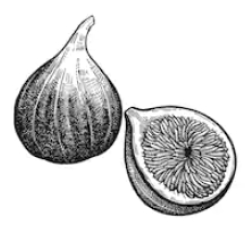
\includegraphics[width=1in,height=1.25in,clip,keepaspectratio]{figures/fig1.png}}]{Orange}
Orange is taste.
\end{IEEEbiography}

\input{private/bio}

\end{document}


